\documentclass[12pt,twoside]{article}
%\usepackage[table]{xcolor} % important to avoid options clash.
%\input{02465shared_preamble}
%\usepackage{cleveref}
\usepackage{url}
\usepackage{graphics}
\usepackage{multicol}
\usepackage{rotate}
\usepackage{rotating}
\usepackage{booktabs}
\usepackage{hyperref}
\usepackage{pifont}
\usepackage{latexsym}
\usepackage[english]{babel}
\usepackage{epstopdf}
\usepackage{etoolbox}
\usepackage{amsmath}
\usepackage{amssymb}
\usepackage{multirow,epstopdf}
\usepackage{fancyhdr}
\usepackage{booktabs}
\usepackage{xcolor}
\newcommand\redt[1]{ {\textcolor[rgb]{0.60, 0.00, 0.00}{\textbf{ #1} } } }


\newcommand{\m}[1]{\boldsymbol{ #1}}
\newcommand{\EE}{\mathbb{E}}
\DeclareMathOperator*{\argmax}{arg\,max}
\DeclareMathOperator*{\argmin}{arg\,min}
\newcommand{\yoursolution}{ \redt{(your solution here) } } 



\title{ Report 2 hand-in }
\date{ \today }
\author{Alen Hodzic (\texttt{s253790}) } 

\begin{document}
\maketitle

\begin{table}[ht!]
\caption{Attribution table}
\begin{tabular}{ll}
\toprule
                                                                    & Alen Hodzic \\
\midrule
 1: Formulate Yodas pendulum as a linear problem                    & 100\%  \\
 2: State at a later time                                           & 100\%  \\
 3: State at a later time II                                        & 100\%  \\
 4: Eigenvalues and powers                                          & 100\%  \\
 5: Analytical expression of Eigenvalues using Euler discretization & 100\%  \\
 6: Bound using Euler discretization                                & 100\%  \\
 7: Matrix norm of Exponential discretization (harder)              & 100\%  \\
 8: Stability                                                       & 100\%  \\
 9: Discretization                                                  & 100\%  \\
 10: Linearization                                                  & 100\%  \\
 11: Unitgrade self-check                                           & 100\%  \\
 12: Control using simple linearization                             & 100\%  \\
 13: MPC                                                            & 100\%  \\
\bottomrule
\end{tabular}
\end{table}

%\paragraph{Statement about collaboration:}
%Please edit this section to reflect how you have used external resources. The following statement will in most cases suffice: 
%\emph{The code in the irls/project1 directory is entirely}

%\paragraph{Main report:}
Headings have been inserted in the document for readability. You only have to edit the part which says \yoursolution. 

\section{Master Yodas pendulum (\texttt{yoda.py})}\label{yoda1}
\subsubsection*{{\color{red}Problem 1:  Formulate Yodas pendulum as a linear problem}}
	
\begin{align}
	A & = \begin{bmatrix}
	0 & 1 \\
	-\frac{g}{L} & 0
	\end{bmatrix} \\
	B & = \begin{bmatrix}
	0 \\
	\frac{1}{mL^2}
	\end{bmatrix}
\end{align}
	\yoursolution 	
	
\subsubsection*{{\color{red}Problem 2:  State at a later time}}
To solve the first part, we proceed by unfolding the recursion. In the absence of input ($\mathbf{B} = 0$, $\mathbf{u} = 0$), the system reduces to
\[
\dot{\mathbf{x}} = A \mathbf{x}.
\]

For Euler discretization we have:
\[
\mathbf{x}_{k+1} = \tilde{A}_0 \mathbf{x}_k, \quad \text{where } \tilde{A}_0 = I + \Delta A
\]

For $N=1$:
\[
\mathbf{x}_1 = \tilde{A}_0 \mathbf{x}_0
\]

For $N=2$:
\[
\mathbf{x}_2 = \tilde{A}_0 \mathbf{x}_1 = \tilde{A}_0^2 \mathbf{x}_0
\]

Continuing this process, we obtain:
\[
\mathbf{x}_N = \tilde{A}_0^N \mathbf{x}_0
\]

Similarly, for exponential integration:
\[
\mathbf{x}_{k+1} = A_0 \mathbf{x}_k, \quad \text{where } A_0 = e^{A\Delta}
\]

For $N=1$:
\[
\mathbf{x}_1 = A_0 \mathbf{x}_0
\]

For $N=2$:
\[
\mathbf{x}_2 = A_0 \mathbf{x}_1 = A_0^2 \mathbf{x}_0
\]

Thus, in general:
\[
\mathbf{x}_N = A_0^N \mathbf{x}_0
\]

As for the second part we get:
\begin{align}
\tilde A_0 & = 
\begin{bmatrix}
1 & \Delta \\
-\frac{g}{L}\Delta & 1
\end{bmatrix}, 
\quad 
A_0 = e^{A\Delta} \approx I + A\Delta + \frac{(A\Delta)^2}{2!} + \cdots \\
& =
\begin{bmatrix}
1 & 0 \\
0 & 1
\end{bmatrix}
+
\begin{bmatrix}
0 & \Delta \\
-\frac{g}{L}\Delta & 0
\end{bmatrix}
+
\frac{1}{2!}
\begin{bmatrix}
-\frac{g}{L}\Delta^2 & 0 \\
0 & -\frac{g}{L}\Delta^2
\end{bmatrix}
+ \cdots
\end{align}
		\yoursolution 	
\subsubsection*{{\color{red}Problem 4:  Eigenvalues and powers}}
	
Let
\[
\tilde{A}_0 = Q \Sigma Q^{-1}, \quad 
\Sigma =
\begin{bmatrix}
\tilde{\lambda}_1 & 0 \\
0 & \tilde{\lambda}_2
\end{bmatrix}.
\]

Then
\[
\tilde{M} = \tilde{A}_0^N = (Q \Sigma Q^{-1})^N.
\]

For $N=2$:
\[
\tilde{A}_0^2 = (Q \Sigma Q^{-1})(Q \Sigma Q^{-1})
= Q \Sigma \underbrace{Q^{-1}Q}_{I} \Sigma Q^{-1}
= Q \Sigma^2 Q^{-1}.
\]

For $N=3$:
\[
\tilde{A}_0^3 = \tilde{A}_0^2 \tilde{A}_0
= (Q \Sigma^2 Q^{-1})(Q \Sigma Q^{-1})
= Q \Sigma^2 \underbrace{Q^{-1}Q}_{I} \Sigma Q^{-1}
= Q \Sigma^3 Q^{-1}.
\]

Continuing this process, we obtain
\[
\tilde{A}_0^N = Q \Sigma^N Q^{-1}.
\]

Since the eigenvectors are orthonormal, we have $Q^{-1} = Q^T$, which ensures that $Q^{-1}Q = I$.

Thus,
\[
\Sigma^N =
\begin{bmatrix}
\tilde{\lambda}_1^N & 0 \\
0 & \tilde{\lambda}_2^N
\end{bmatrix},
\]

and therefore the eigenvalues of $\tilde{M}$ are $\tilde{\lambda}_1^N$ and $\tilde{\lambda}_2^N$.
\yoursolution
	
\subsubsection*{{\color{red}Problem 5:  Analytical expression of Eigenvalues using Euler discretization}}

We compute the eigenvalues from the characteristic equation
\[
\det(\tilde{A}_0 - \lambda I) = 0.
\]

This gives
\[
\det
\begin{bmatrix}
1 - \lambda & \Delta \\
-\frac{g}{L}\Delta & 1 - \lambda
\end{bmatrix}
= (1 - \lambda)^2 + \frac{g}{L}\Delta^2 = 0.
\]

Solving for $\lambda$ yields
\[
\lambda_{1,2} = 1 \mp i \Delta \sqrt{\frac{g}{L}}.
\]
\yoursolution

\subsubsection*{{\color{red}Problem 6:  Bound using Euler discretization}}

Using Euler discretization we get the upper bound:
$$
\| \mathbf{x}_N \| = \| \tilde{A}_0^N \mathbf{x}_0 \| 
\leq \| \tilde{A}_0^N \|
= \| \tilde{A}_0 \|^N 
= \left( \max |\lambda_i| \right)^N 
= \left(\sqrt{1 + \frac{g}{L}\Delta^2}\right)^N,
$$
where we used that $\|\mathbf{x}_0\| = 1$ and the matrix norm definition
$$
\|A\| = \max_{\|x\|=1} \|Ax\|.
$$
\yoursolution
	
\subsubsection*{{\color{red}Problem 7:  Matrix norm of Exponential discretization (harder)}}
	
Using exponential integration we get
$$
\| \mathbf{x}_N \| = \| A_0^N \mathbf{x}_0 \| 
\leq \| A_0^N \|
= \| A_0 \|^N,
$$
where we used that $\|\mathbf{x}_0\| = 1$.

We now compute the eigenvalues of $A_0 = e^{\Delta A}$. First compute the eigenvalues of $\Delta A$:
\[
\Delta A =
\begin{bmatrix}
0 & \Delta \\
-\frac{g}{L}\Delta & 0
\end{bmatrix}.
\]

The characteristic equation is
\[
\det(\Delta A - \lambda I) = \lambda^2 + \frac{g}{L}\Delta^2 = 0,
\]
which gives
\[
\lambda = \pm i \sqrt{\frac{g}{L}} \Delta.
\]

We now use the eigendecomposition $\Delta A = Q \Sigma Q^{-1}$, where
\[
\Sigma =
\begin{bmatrix}
\lambda_1 & 0 \\
0 & \lambda_2
\end{bmatrix}.
\]

Using the definition of the matrix exponential,
\[
e^{\Delta A} = I + \Delta A + \frac{(\Delta A)^2}{2!} + \cdots,
\]
and the fact that $(\Delta A)^n = Q \Sigma^n Q^{-1}$, we obtain
\[
e^{\Delta A}
= Q \left( I + \Sigma + \frac{\Sigma^2}{2!} + \cdots \right) Q^{-1}
= Q e^{\Sigma} Q^{-1}.
\]

Since $\Sigma$ is diagonal, we have
\[
e^{\Sigma} =
\begin{bmatrix}
e^{\lambda_1} & 0 \\
0 & e^{\lambda_2}
\end{bmatrix}.
\]

Thus, the eigenvalues of $A_0 = e^{\Delta A}$ are
\[
\lambda_{1,2} = e^{\pm i \sqrt{\frac{g}{L}} \Delta}.
\]

Since $|e^{i\theta}| = 1$, it follows that
\[
\|A_0\| = \max |\lambda_i| = 1.
\]

Therefore,
$$
\| \mathbf{x}_N \| \leq 1.
$$
		\yoursolution
	
\section{R2D2 and control (\texttt{r2d2.py})}
\subsubsection*{{\color{red}Problem 9:  Discretization}}

$$
\m x_{k+1} = \m f_k(\m x_k, \m u_k) =
\begin{bmatrix}
x_k + \Delta v_k \cos(\gamma_k) \\
y_k + \Delta v_k \sin(\gamma_k) \\
\gamma_k + \Delta \omega_k
\end{bmatrix}
$$

\subsubsection*{{\color{red}Problem 10:  Linearization}}
	
$$
\m x_{k+1} \approx 
\begin{bmatrix}
1 & 0 & -\Delta \sin\theta \\
0 & 1 & \Delta \cos\theta \\
0 & 0 & 1
\end{bmatrix} \m x_k +
\begin{bmatrix}
\Delta \cos\theta & 0 \\
\Delta \sin\theta & 0 \\
0 & \Delta
\end{bmatrix} \m u_k +
\begin{bmatrix}
\Delta \theta \sin\theta \\
-\Delta \theta \cos\theta \\
0
\end{bmatrix}
$$
	
\subsubsection*{{\color{red}Problem 12:  Control using simple linearization}}
			
		% Just generate the figures using the script and change the path below. 
		\begin{center}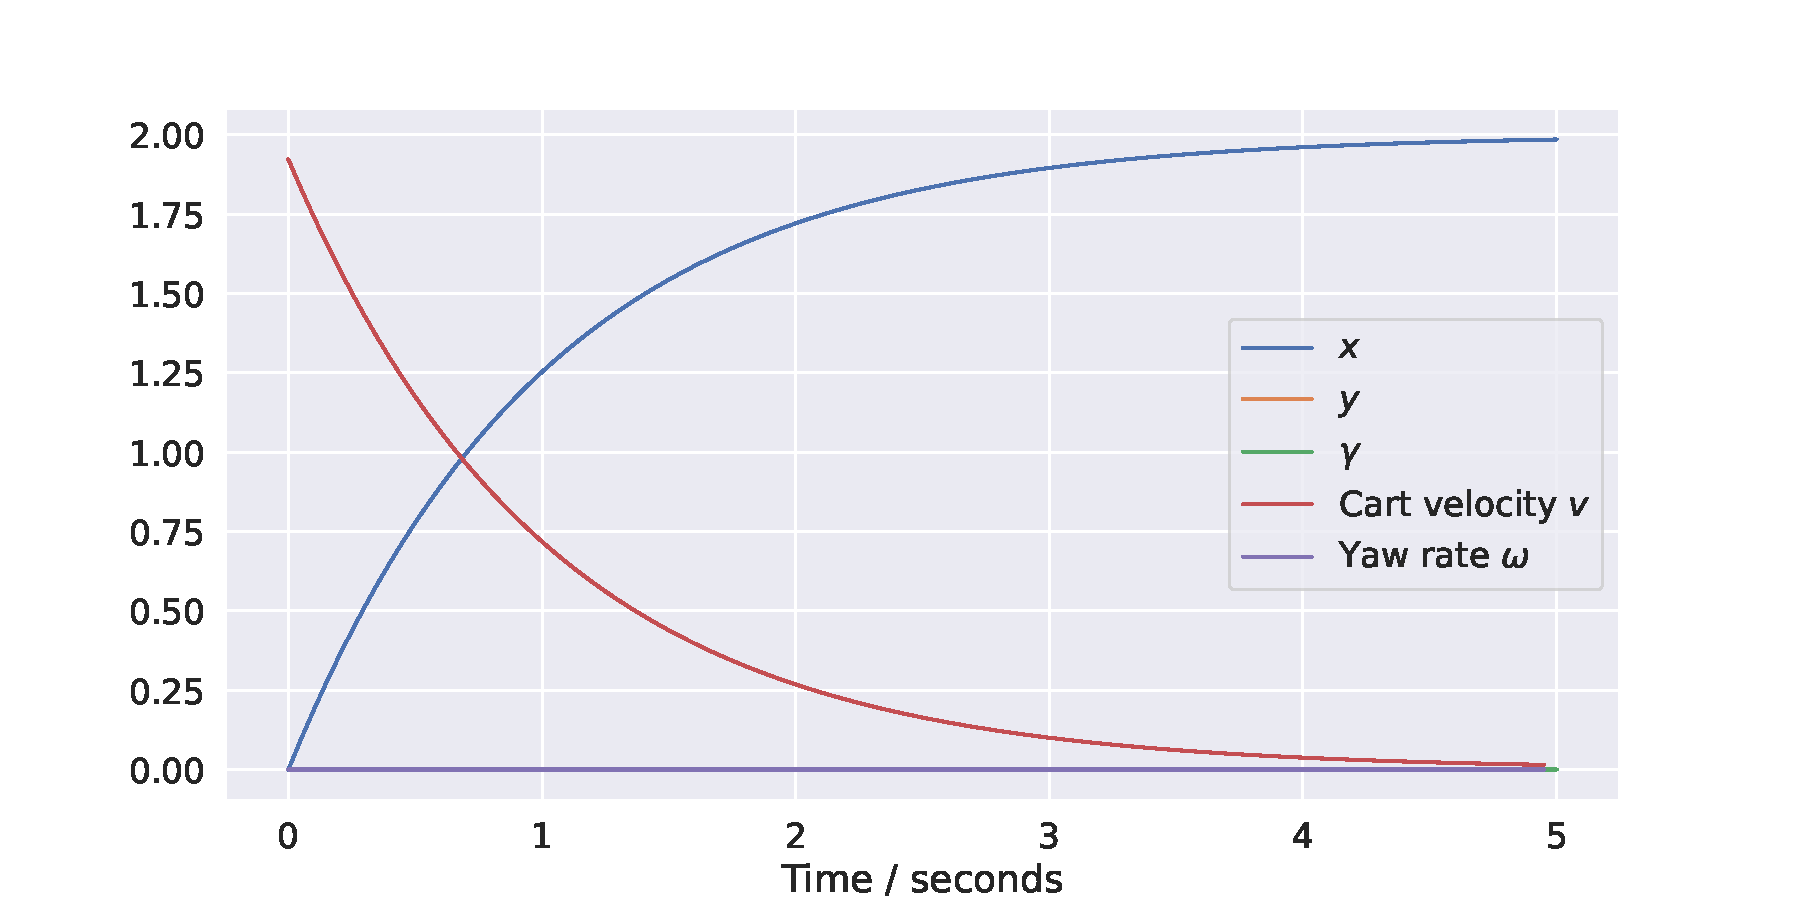
\includegraphics[width=.5\linewidth]{figures/r2d2_linearization_1.pdf}~
		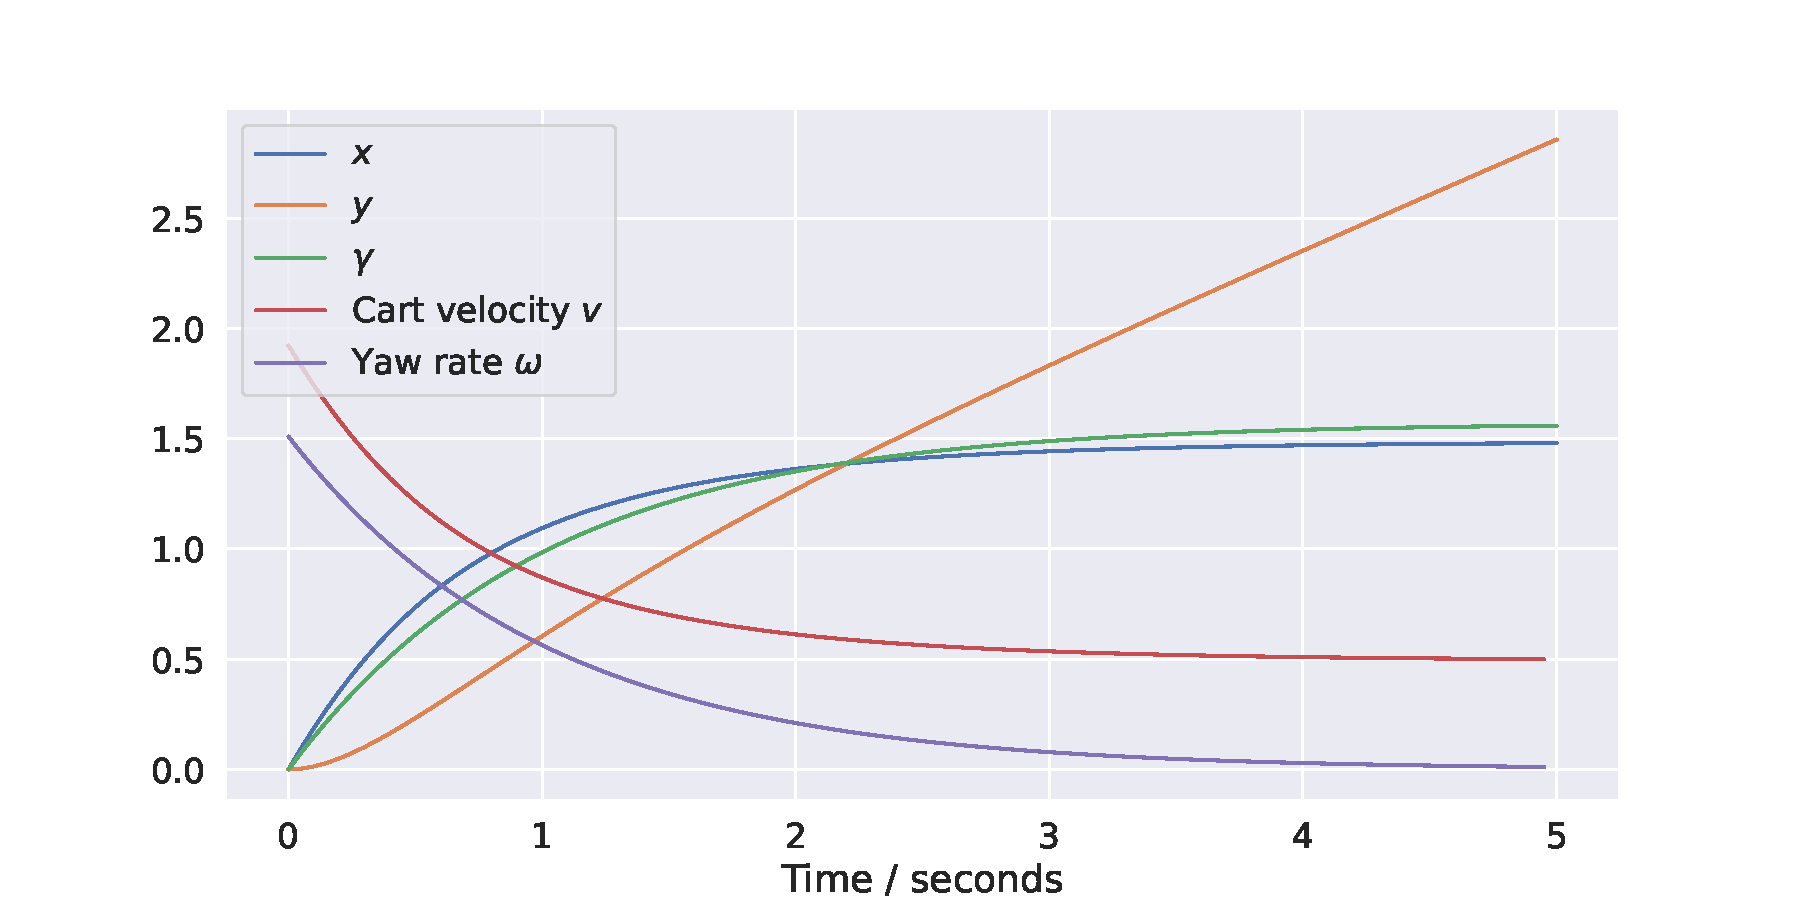
\includegraphics[width=.5\linewidth]{figures/r2d2_linearization_2.pdf} \end{center}
The system is linearized around the fixed point $\bar{x}=0$, $\bar{u}=0$.

For $x^* = [2,0,0]^T$, the motion remains close to $\gamma \approx 0$, where $\sin(\gamma) \approx 0$ and $\cos(\gamma) \approx 1$. Hence, the linear approximation is accurate and the controller performs well.

For $x^* = [2,2,\frac{\pi}{2}]^T$, the system must reach $\gamma = \frac{\pi}{2}$, where $\sin(\gamma)=1$ and $\cos(\gamma)=0$. This is far from the linearization point, and the approximation $\sin(\gamma) \approx 0$, $\cos(\gamma) \approx 1$ becomes invalid.\yoursolution	
	
\subsubsection*{{\color{red}Problem 13:  MPC}}
			
		\begin{center}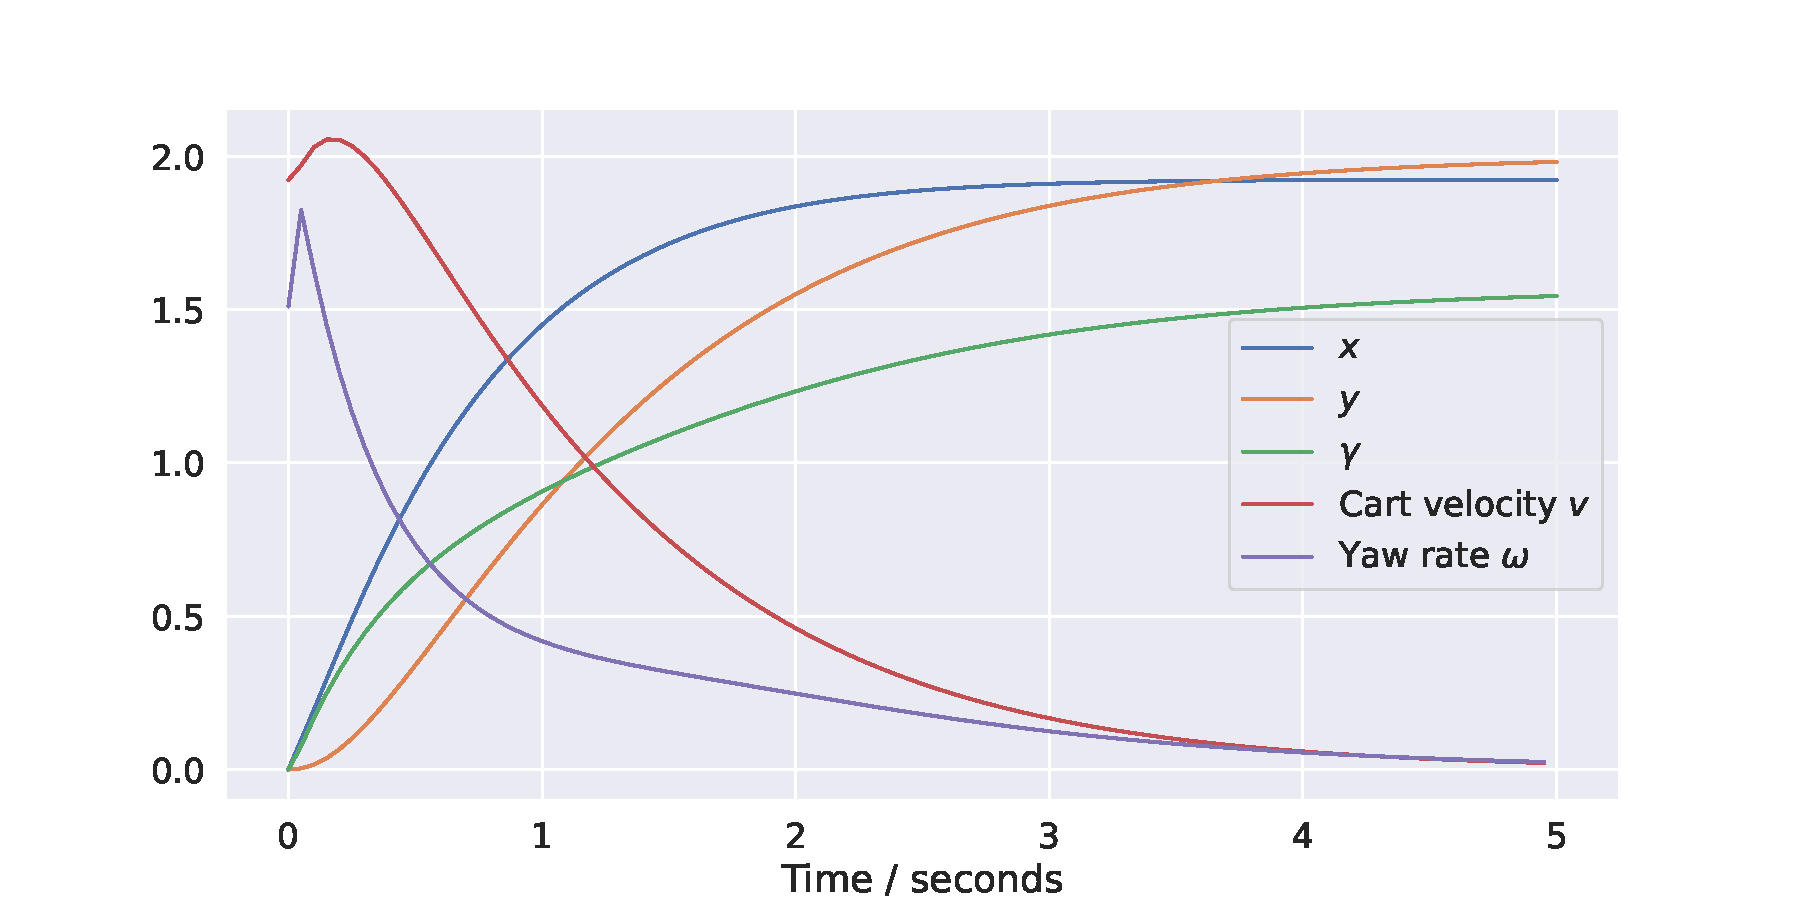
\includegraphics[width=.6\linewidth]{figures/r2d2_iterative_1.pdf}%~
		%	
\includegraphics[width=.5\linewidth]{figures/your_answer} 
	\end{center}
		In iterative linearization, the system is re-linearized at each time step around the current state and previous control. This means the linear model is always a local approximation of the true nonlinear dynamics.

As a result, the controller continuously adapts to the current state, capturing changes in orientation and position more accurately. In particular, the nonlinear effects of $\sin(\gamma)$ and $\cos(\gamma)$ are better approximated since the linearization point moves with the system.\yoursolution
	
\end{document}